\section{Jeffreson Correction to Lumped Capacitance Method}\label{sec:ht-jeffreson-correction}
When incorporating helium into the DEM-based modeling, the lumped capacitance assumption for each particle in the ensemble is assumed. The assumption eases the computational efforts of solving for the temperature distribution inside each particle; each particle is treated as being isothermal. The accuracy of the lumped capacitance method is described by the Biot number,
\begin{equation}
     \Bi = \frac{hd_p}{k_r}
\end{equation} 
and for $\Bi \ll 1$ the lumped capacitance method accurately models the behavior of a solid interacting with a fluid. For $\Bi \approx 0.1$ (in cases with no heat generation), the error from the lumped capacitance method is only about 5\%. In solid breeder volumes, the particles are generally small, the solid conductivity low, and heat transfer coefficient generally is also low. This leads to small-to-moderate Biot numbers expected in the packed bed. In this section we will analyze the accuracy of the lumped capacitance and introduce a correction method to account for inaccuracies of the method at moderate Biot numbers.

I simplify the case of a packed bed and only consider a single sphere with volumetric heat generation submerged in- and thermally interacting with a fluid. The sphere will be of radius $R=d_p/2$, as shown in Fig.~\ref{fig:ParticleControlVolume}. The sphere will initially be at a uniform temperature of $T_i$. The fluid temperature will remain constant at $T_f$

\begin{figure}[ht]
	\centering
		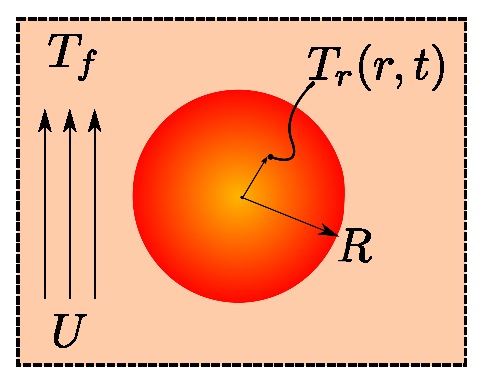
\includegraphics[width=2in]{chapters/figures/ParticleControlVolume}
	\caption[Control volume of single spherical particle in a packed bed]{Control volume of a single spherical particle in a packed bed}
	\label{fig:ParticleControlVolume}
\end{figure}


%~~~~~~~~~~~~~~~~~~~~~~~~~~~~~~~~~~~~~~~~~~~~~~~~~~~~~~~
\subsection{Lumped Capacitance Solution for Sphere}\label{sec:lumped-capacitance}
I solve for a single sphere interacting with a passing fluid, as shown in Fig.~\ref{fig:ParticleControlVolume}, while making the lumped capacitance assumption for this sphere. The solid is initially at temperature $T_0$, with constant volumetric heat generation, cooling in a fluid with constant heat transfer coefficient. The fluid will remain constant at $T_f$.

The time response of the sphere's temperature is dictated by the balance of energy to/away from the solid,  

\begin{equation}\label{eq:lc-energy-balance}
	\rho_rC_rV\frac{dT}{dt} = -hA(T-T_f) + \dot{g}V
\end{equation}

Eq.~\ref{eq:lc-energy-balance} is solved in dimensionless form with the following nondimensional parameters of temperature and time,
\begin{subequations}
\begin{align}
    \theta &= \frac{T(t) - T_f}{T_0 - T_f}\\
    \tau & = \frac{t}{R^2/\alpha}
\end{align}
\end{subequations}
where $\alpha$ is the thermal diffusivity of the sphere, $T_0$ is the initial isothermal temperature of the sphere, and $T_f$ is the constant fluid temperature. The resulting temperature distribution is,
\begin{equation}
\label{eq:theta-lc}
	\theta_{LC}=\left(1-\frac{G}{3\Bi}\right)\exp(-3\Bi \tau) + \frac{G}{3\Bi}
\end{equation}
where I have defined a dimensionless heat generation,
\begin{equation}\label{eq:nondimensional-heat-generation}
	G = \frac{\dot{g}R^2}{k(T_0 - T_f)}
\end{equation}

The energy contained in the sphere, relative to the fluid, in nondimensional terms is 
\begin{equation}
    E^*(\tau)=\frac{E(\tau)}{E_0}
\end{equation}
where $E_0$ is the initial energy of the sphere,
\begin{equation}
    E_0=\rho_rC_rV(T_0-T_f)
\end{equation}

Thus for a sphere with the lumped capacitance model, in nondimensional form, the energy is simply
\begin{equation}\label{eq:lc-energy-profile}
	E^*_{LC}(\tau) = \theta_{LC}(\tau) = \left(1-\frac{G}{3\Bi}\right)\exp(-3\Bi \tau) + \frac{G}{3\Bi}
\end{equation}

The nondimensional energy profile of Eq.~\ref{eq:lc-energy-profile} is plotted over the nondimensional time of $\tau \in [0,1/\Bi]$ in Fig.~\ref{fig:LC-sphere-in-fluid}. 

\begin{figure}[ht]
	\centering
		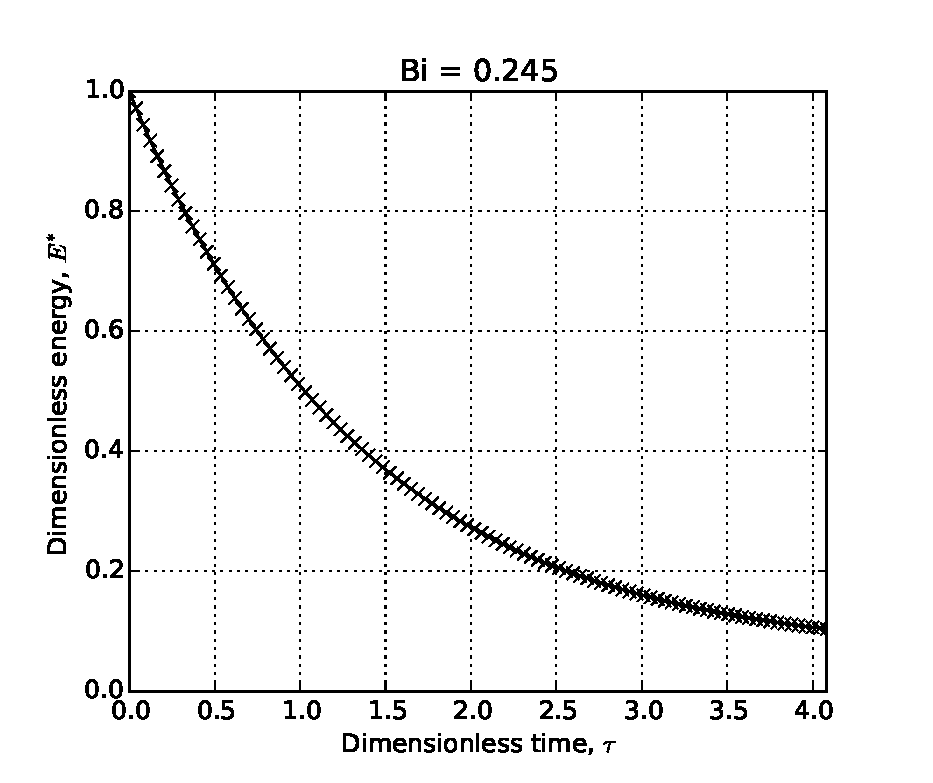
\includegraphics[width=\singleimagewidth]{chapters/figures/LC-sphere-in-fluid}
	\caption[Lumped Capacitance energy profile]{Lumped capacitance model: Sphere energy profile decaying from an initial value to a time of $1/\Bi$}
	\label{fig:LC-sphere-in-fluid}
\end{figure}

Reviewing Eq.~\ref{eq:theta-lc} we see that the speed of decay is dictated by the term in the exponential, $3\Bi$. Meanwhile, the steady-state value being approached is given by $\frac{G}{3\Bi} = \frac{gR}{h(T_0 - T_f)}$. It is important for this discussion to point out that because both the nondimensional heat generation and Biot number terms contain the solid conductivity, the steady-state value of the lumped capacitance model will not change for varying solid conductivity even if it leads to different Biot numbers. I will return to this point in the next section when comparing the lumped capacitance model to the exact solution when internal conduction of the solid is considered.
%~~~~~~~~~~~~~~~~~~~~~~~~~~~~~~~~~~~~~~~~~~~~~~~~~~~~~~~



%~~~~~~~~~~~~~~~~~~~~~~~~~~~~~~~~~~~~~~~~~~~~~~~~~~~~~~~
\subsection{Exact Solution for Sphere}\label{sec:analytic-sphere}

I again analyze the sphere of Fig.~\ref{fig:ParticleControlVolume} but now will account for internal temperature gradients inside the sphere. The details of the analytic solution for a sphere with heat generation interacting with a fluid is given in Appendix~\ref{sec:analytic-sphere-details}. Again, solving in terms of the nondimensional temperature and time introduced in \cref{sec:lumped-capacitance} as well as a nondimensional radius,

\begin{align*}
    \theta &= \frac{\mathbb{T}}{\mathbb{T}_0}\\
    \rho & = \frac{r}{R}\\
    \tau & = \frac{t}{R^2/\alpha}
\end{align*}

The energy conservation equation for the sphere with internal temperature gradient, in nondimensional form $\theta_{TG}$, is
\begin{equation}
    \frac{1}{\rho}\frac{\partial^2}{\partial \rho^2}(\rho\theta_{TG}) + G = \frac{\partial\theta_{TG}}{\partial \tau}
\end{equation}

With the initial condition and boundary conditions outlined in \cref{sec:analytic-sphere-details}, the nondimensional temperature distribution inside the sphere is 
\begin{equation}\label{eq:analytic-temperature-distribution}
    \theta_{TG}(\rho,\tau) = \left(\frac{G}{6} + \frac{G}{3\Bi}-\rho^2\right)  +   \sum_{n=1}^\infty \exp(-\zeta^2 \tau) \frac{\sin(\zeta_n \rho)}{\rho} \frac{Z(\zeta_n)}{N(\zeta_n)}  
\end{equation}
where $\zeta_n$ are the eigenvalues of the equation and the functions of $\zeta_n$ ($Z$,$N$,$C$) are given in \cref{sec:analytic-sphere-details}.

The accompanying nondimensional energy of the sphere is integrated to,
\begin{equation}
\label{eq:analytic-energy-profile}
    E^*_{TG}(\tau)=\left(\frac{G}{15}+\frac{G}{3\Bi}\right)+3\sum_{n=1}^\infty \exp(-\zeta^2 \tau) \frac{Z(\zeta_n)}{N(\zeta_n)} C_n(\zeta_n)
\end{equation}

I now compare the exact solution from Eq.~\ref{eq:analytic-energy-profile} to the solution of energy given by the lumped capacitance model of Eq.~\ref{eq:lc-energy-profile}. The two profiles are given in Fig.~\ref{fig:LC-analytic-sphere-in-fluid}. 

\begin{figure}[ht]
	\centering
		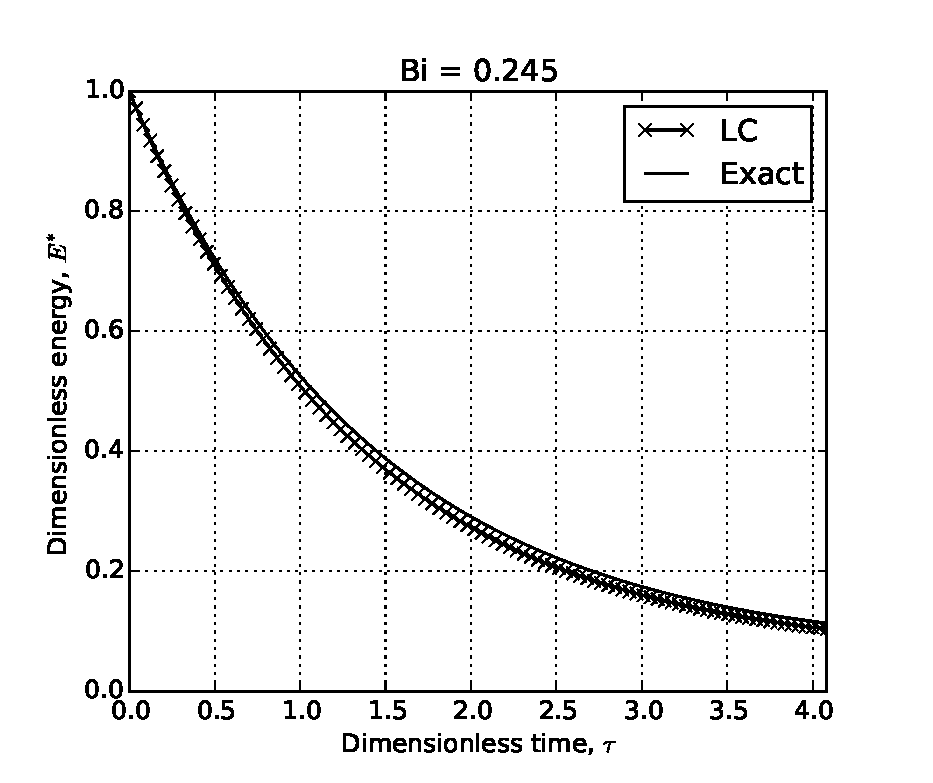
\includegraphics[width=\singleimagewidth]{chapters/figures/LC-analytic-sphere-in-fluid}
	\caption[Analytic temperature profile for $\Bi < 1$]{Analytic and lumped capacitance models: Sphere energy profile decaying from an initial value to a time of $1/\Bi$}
	\label{fig:LC-analytic-sphere-in-fluid}
\end{figure}

For the value of Biot number here, $\Bi = 0.245$, the energy profile of the analytic solution of the sphere cooling in a flow is well-captured by the lumped capacitance model. The maximum relative error over the time span, as defined by
\begin{equation}\label{eq:error}
	\text{error} = \frac{\big|E^*_{TG}(\tau) - E^*_{LC}(\tau) \big|}{E^*_{TG}(\tau)}
\end{equation}
is always less than 10\%. 

Consider now the same size sphere but with the Biot number increased by an order from: a) a conductivity of $k = k_r/10$ and b) a heat transfer coefficient of $h = 10h_f$. The two physical changes to the system result in the same Biot number ($\Bi = 2.45$) but as we can see in Fig.~\ref{fig:LC-analytic-sphere-in-fluid-Bi-2}, there are drastic differences between the energy profiles.

\begin{figure}
        \centering
        \begin{subfigure}[b]{0.5\textwidth}
                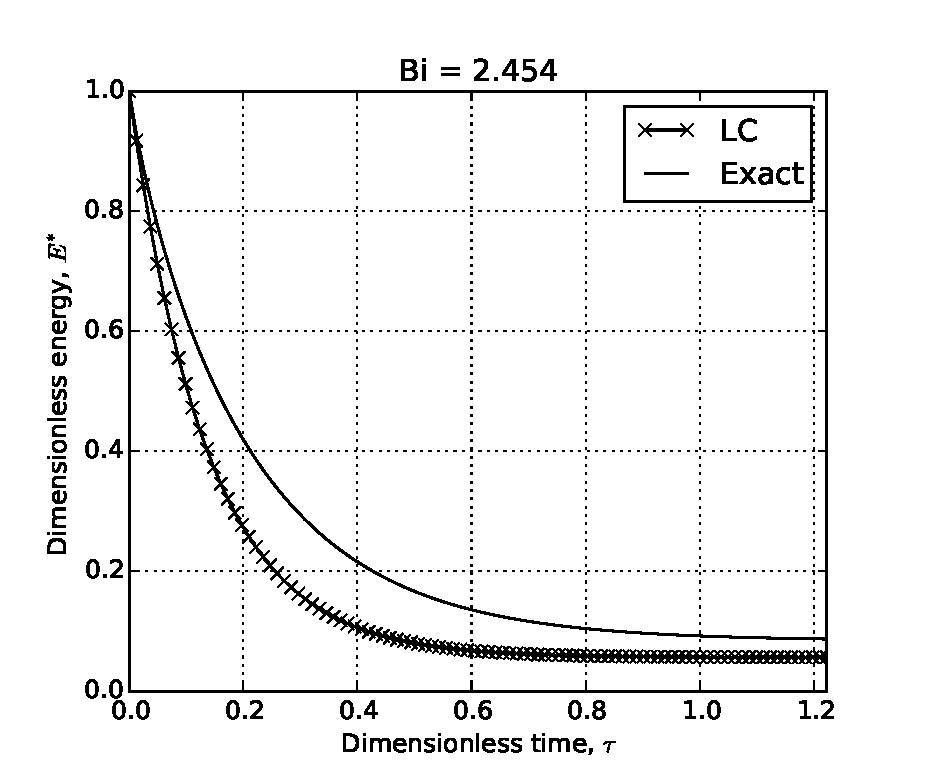
\includegraphics[width=\textwidth]{chapters/figures/LC-analytic-sphere-in-fluid-Bi-2a}
                \caption{$k \uparrow$, lumped capacitance error in the transient and steady-state.}
				\label{fig:LC-analytic-sphere-in-fluid-Bi-2a}
        \end{subfigure}%
        
          %add desired spacing between images, e. g. ~, \quad, \qquad, \hfill etc.
          %(or a blank line to force the subfigure onto a new line)
        \begin{subfigure}[b]{0.5\textwidth}
                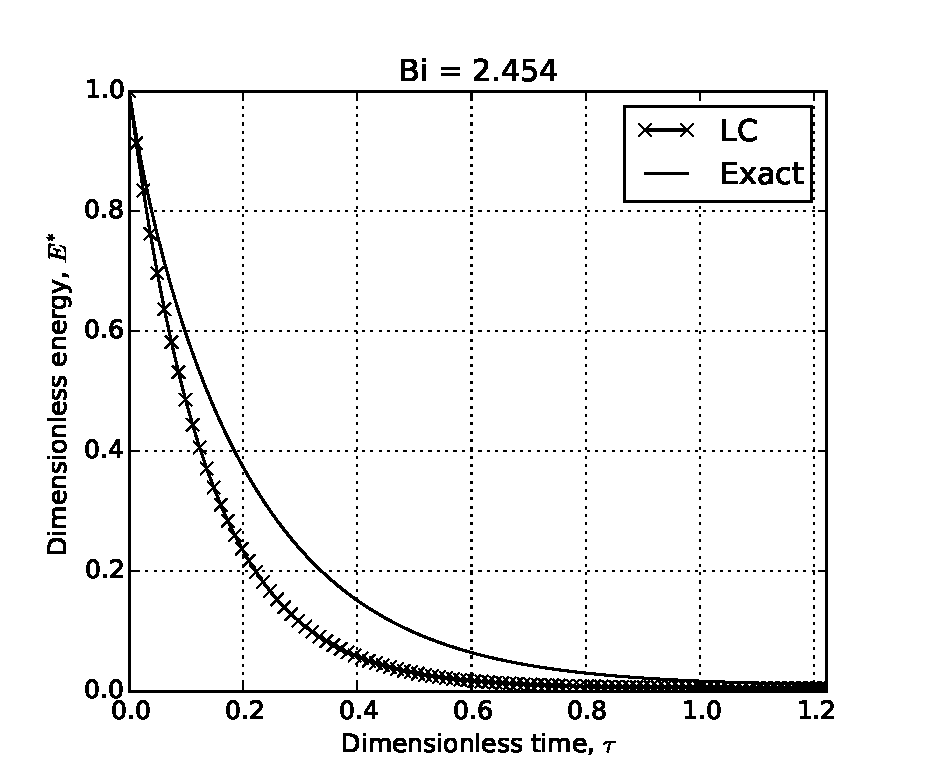
\includegraphics[width=\textwidth]{chapters/figures/LC-analytic-sphere-in-fluid-Bi-2b}
                \caption{$h \uparrow$, lumped capacitance error mainly in the transient.}
				\label{fig:LC-analytic-sphere-in-fluid-Bi-2b}
        \end{subfigure}
        \caption[Analytic temperature profile for moderate Biot number]{Analytic and lumped capacitance models: Sphere energy profile decaying from an initial value to a time of $3/\Bi$. The same Biot number produces different results for the exact solution of a sphere with heat generation.}\label{fig:LC-analytic-sphere-in-fluid-Bi-2}
\end{figure}

Seen in Fig.~\ref{fig:LC-analytic-sphere-in-fluid-Bi-2a}, the lumped capacitance solution both over-predicts the speed at which the sphere reaches a thermal steady-state as well as the value of the steady-state. Comparatively, in Fig.~\ref{fig:LC-analytic-sphere-in-fluid-Bi-2b}, for the same Biot number, the lumped capacitance solution again over-predicts the speed to thermal steady-state by the same rate but is relatively accurate for the steady-state value itself. 

Viewing the steady-state terms of the two solutions, the source of the error becomes apparent. From Eq.~\ref{eq:analytic-energy-profile}, the steady-state term of the exact solution is
\begin{equation}
	E^*_{TG,ss}=\frac{G}{15}+\frac{G}{3\Bi}
\end{equation}

Whereas, the steady-state term of the lumped capacitance solution from Eq.~\ref{eq:lc-energy-profile} is,
\begin{equation}
	E^*_{LG,ss} = \frac{G}{3\Bi}
\end{equation}

The two steady-state values differ only by the additional term of $\frac{G}{15}$ on the exact solution. This term appears in the exact solution from integration of the temperature gradient that exists in the pebble due to volumetric heating (see \cref{sec:analytic-sphere-details}). The lumped capacitance solution assumes no internal temperature gradient in the sphere and thus by definition can not account for this $\frac{G}{15}$ term. Furthermore, the nondimensional heat generation term, $G$, given in Eq.~\ref{eq:nondimensional-heat-generation}, is importantly a function of thermal conductivity but not the heat transfer coefficient. The lack of dependence on $h$ explains the difference between steady-state values in Fig.~\ref{fig:LC-analytic-sphere-in-fluid-Bi-2}. When $\Bi$ is small, the steady state error between lumped capacitance and the exact solution is small. If only $h$ increases the error in steady-state remains small. This is demonstrated in Fig.~\ref{fig:LC-analytic-error-Bi-2b} when steady-state solutions are close. However, in Fig.~\ref{fig:LC-analytic-sphere-in-fluid-Bi-2a} as $k$ was reduced, the curves no longer converge to similar steady-states. This phenomena appears only with the combination of low conductivity materials with volumetric heating.

Even in cases without volumetric heating, when the Biot number grows large, errors appear in the transient portion of curves but ultimately converge to the same steady-state solutions. To address the inaccuracies in the time-dependent response of the lumped capacitance method with large Biot number, I make use a a correction factor such as that used by Van Lew and Xu\etal where they implemented the correction in situations without heat generation.\cite{VanLew2010,Xu2012}. In their work, they considered a heat transfer fluid interacting with a low conductivity thermal storage material. The solar thermal storage systems they analyzed often had moderate-to-large Biot numbers but they could continue to apply the lumped capacitance model in their calculations with application of a so-called Jeffreson Correction.\cite{jeffreson409} However, because their applications did not involve heat generation, I must validate its usefulness for application in our pebble beds absorbing nuclear heat.
%~~~~~~~~~~~~~~~~~~~~~~~~~~~~~~~~~~~~~~~~~~~~~~~~~~~~~~~





%~~~~~~~~~~~~~~~~~~~~~~~~~~~~~~~~~~~~~~~~~~~~~~~~~~~~~~~
\subsection{Jeffreson Correction for Sphere with Nuclear Heating}
The correlation to correct the heat transfer coefficient due to solids with large Biot number is given by Jeffreson as,\cite{jeffreson409}
\begin{equation}
	h_{p}=\frac{h}{1+\Bi/5}
\end{equation}
where $h_p$ is the modified heat transfer coefficient of the particle with an internal temperature gradient. As the Biot number increases, the modified heat transfer coefficient decreases. THe form of this correlation works to effectively slow down the rate of heat removed by the passing fluid. Recall the curves of Fig~\ref{fig:LC-analytic-sphere-in-fluid-Bi-2}. where the lumped capacitance solution over-predicted the speed with which the energy decayed towards steady-state. A modified Biot number can then also be written as
\begin{equation}\label{eq:jeffreson-correction-bip}
	\Bi_p = \frac{h_p d}{k_r} = \frac{\Bi}{1+\Bi/5}
\end{equation}

Applying the Jeffreson Correction to Eq.~\ref{eq:theta-lc}, the modified lumped capacitance solution is written now in terms of the modified Biot number,
\begin{equation}
\label{eq:theta-jc-bip}
	\theta_{JC}=\left(1-\frac{G}{3\Bi_p}\right)\exp\left(-3\Bi_p \tau\right) + \frac{G}{3\Bi_p}
\end{equation}
and thereby Eq.~\ref{eq:lc-energy-profile} also yields
\begin{equation}\label{eq:jc-energy-profile}
	E^*_{JC}(\tau) = \left(1-\frac{G}{3\Bi_p}\right)\exp\left(-3\Bi_p \tau\right) + \frac{G}{3\Bi_p}
\end{equation}

The energy profiles from the lumped capacitance model (LC), the Jeffreson correction (JC), and the exact solution are all plotted together in Fig.~\ref{fig:LC-JC-analytic-sphere-in-fluid-Bi-2}. Barely visible under the JC solution are teh curves from the exact solution. The Jeffreson correction to the lumped capacitance method allows the simple modeling approach of the lumped capacitance method to capture the proper transient as well as steady-state values for this sphere with a moderately sized Biot number. 

\begin{figure}
        \centering
        \begin{subfigure}[b]{0.5\textwidth}
                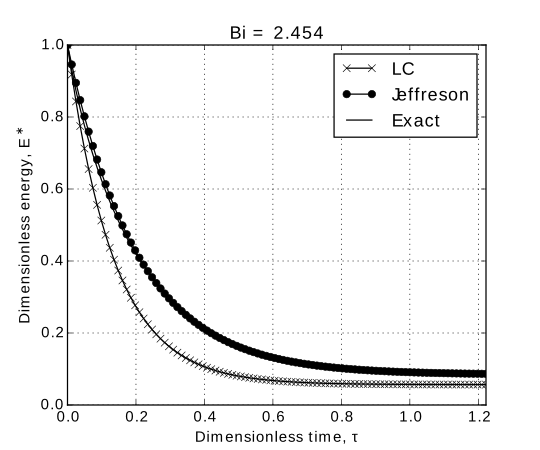
\includegraphics[width=\textwidth]{chapters/figures/LC-JC-analytic-sphere-in-fluid-Bi-2a}
                \caption{The Biot number increased from a decrease in the solid conductivity.}
				\label{fig:LC-JC-analytic-sphere-in-fluid-Bi-2a}
        \end{subfigure}%
        
          %add desired spacing between images, e. g. ~, \quad, \qquad, \hfill etc.
          %(or a blank line to force the subfigure onto a new line)
        \begin{subfigure}[b]{0.5\textwidth}
                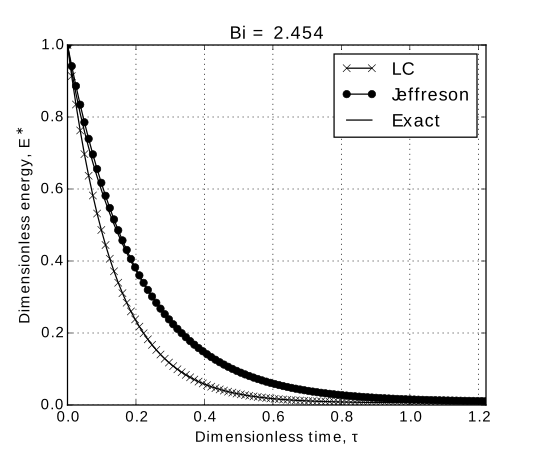
\includegraphics[width=\textwidth]{chapters/figures/LC-JC-analytic-sphere-in-fluid-Bi-2b}
                \caption{The Biot number increased from  an increase in the heat transfer coefficient.}
				\label{fig:LC-JC-analytic-sphere-in-fluid-Bi-2b}
        \end{subfigure}
        \caption[Jeffreson correction for moderate Biot number based on conductivity]{Analytic, lumped capacitance model, and LC model with Jeffreson correction: Jeffreson correction corrects for transient and steady-state errors of lumped capacitance.}\label{fig:LC-JC-analytic-sphere-in-fluid-Bi-2}
\end{figure}

\begin{figure}
        \centering
        \begin{subfigure}[b]{0.5\textwidth}
                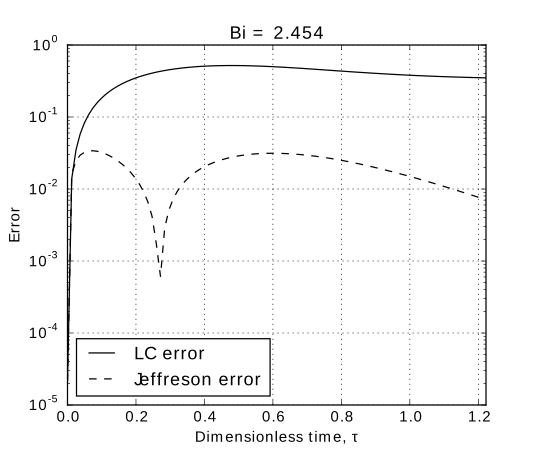
\includegraphics[width=\textwidth]{chapters/figures/LC-JC-analytic-error-Bi-2a}
                \caption{The Biot number increased from a decrease in the solid conductivity.}
				\label{fig:LC-JC-analytic-error-Bi-2a}
        \end{subfigure}%
        
          %add desired spacing between images, e. g. ~, \quad, \qquad, \hfill etc.
          %(or a blank line to force the subfigure onto a new line)
        \begin{subfigure}[b]{0.5\textwidth}
                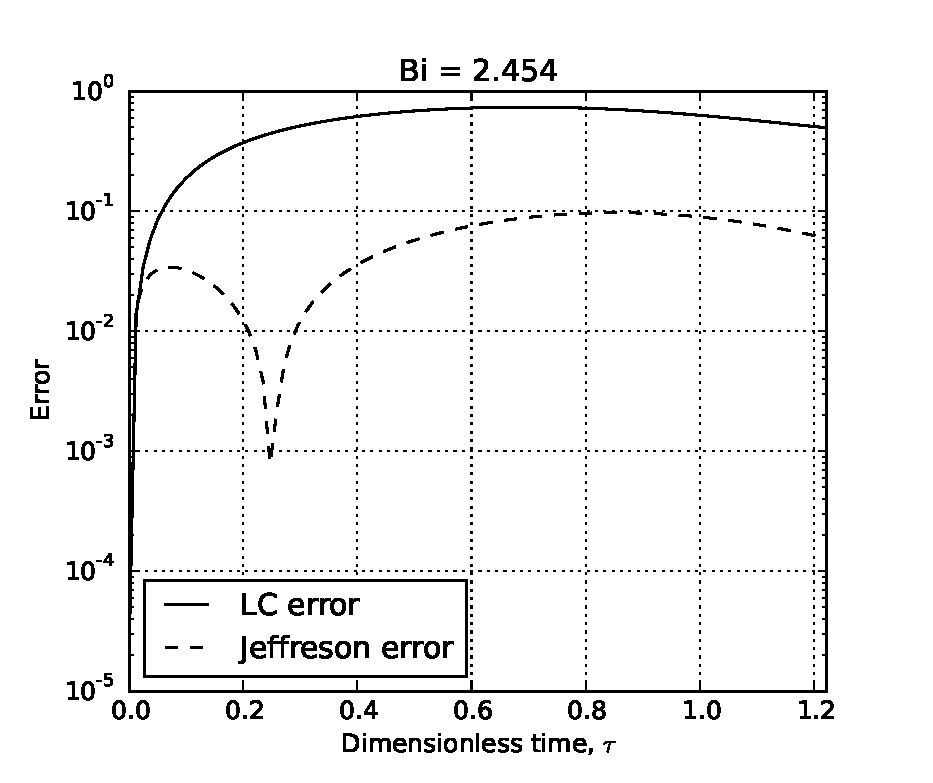
\includegraphics[width=\textwidth]{chapters/figures/LC-JC-analytic-error-Bi-2b}
                \caption{The Biot number increased from  an increase in the heat transfer coefficient.}
				\label{fig:LC-JC-analytic-error-Bi-2b}
        \end{subfigure}
        \caption[Error of lumped capacitance and Jeffreson correction for moderate Biot number]{Error of lumped capacitance and reduced error of the model with Jeffreson correction for moderate Biot number.}\label{fig:LC-JC-analytic-error-Bi-2}
\end{figure}

To look more closely, we view the instantaneous error (see Eq.~\ref{eq:error}) in Fig.~\ref{fig:LC-JC-analytic-error-Bi-2}. For the value of $\Bi > 1$ due to either low conductivity (Fig.~\ref{fig:LC-JC-analytic-error-Bi-2a}) or high heat transfer coefficient (Fig.~\ref{fig:LC-JC-analytic-error-Bi-2b}), the error in the Jeffreson correction is always under 10\%; often closer to only 1\%. This is in opposition to the standard lumped capacitance method which has 50-80\% error for both transient and steady-state values.

The lumped capacitance method allows researchers to simplify transient, conjugate heat transfer problems to a situation with an isothermal solid. In the discrete element method, the assumption of isothermal solid is innate in the framework of the method. With the implementation of the Jeffreson correction in the discrete element method, we have confidence in the fidelity of the heat transfer with the helium flow for moderately sized Biot numbers. The Jeffreson correction will be implemented into the DEM computations via Eq.~\ref{eq:jeffreson-correction-bip}. 
%~~~~~~~~~~~~~~~~~~~~~~~~~~~~~~~~~~~~~~~~~~~~~~~~~~~~~~~